This section describes the processes and steps that our team took to study the data.

\subsection{Describe provided data}

The provided data resides inside two parent directories:

\begin{verbatim}
    data
    |--- convert
    |--- UF
\end{verbatim}

For the \texttt{convert} directory, it seems like the data there has been converted from the other \texttt{UF} files.
Compared with the original, these files do not store as many necessary fields,
with many meteorologist features being left out or not included.
For instance, fields like \textbf{Reflectivity}, \textbf{Mean doppler velocity} and \textbf{Doppler spectrum width} only appear
in the \texttt{UF} files, but not in the converted ones.

\begin{lstlisting}[language=python,caption={A sample of metadata extracted from UF file}]
{
    'time': {
        'units': 'seconds since 2019-05-13T01:20:07Z',
    }
    ...
    'fields': {
        'total_power': {
            'units': 'dBZ',
            'standard_name': 'equivalent_reflectivity_factor',
            'long_name': 'Total power',
            'coordinates': 'elevation azimuth range',
            'data': masked_array(
                data=[
                    [37.0, 27.5, 37.5, ..., --, --, --],
                    [50.0, 41.0, 31.5, ..., --, --, --],
                    [45.0, 41.0, 29.5, ..., 0.0, 4.0, 7.0],
                    ...,
                    [35.0, 32.0, 21.0, ..., 3.0, --, --],
                    [33.5, 27.5, 20.0, ..., --, --, --],
                    [41.0, 31.5, 27.0, ..., --, --, --]
                ],
                mask=[
                    [False, False, False, ...,  True,  True,  True],
                    [False, False, False, ...,  True,  True,  True],
                    [False, False, False, ..., False, False, False],
                    ...,
                    [False, False, False, ..., False,  True,  True],
                    [False, False, False, ...,  True,  True,  True],
                    [False, False, False, ...,  True,  True,  True]
                ],
                fill_value=1e+20,
                dtype=float32
            ),
            '_FillValue': -9999.0
        },
    ...
    }
}
\end{lstlisting}


As a result, we decided to use the \texttt{UF} files for our study, while temporarily ignoring the \texttt{convert} directory.


\subsection{Comparing PyART and LROSE}
From the advice of our professor, at first, we decided to learn about LROSE and try to open the provided data.
LROSE is a set of multiple tools and libraries for working with Radar data output.
For macOS, support for Homebrew makes it easier to install these tools for local usage.
However, for other platforms, downloading and compiling the source code is required,
which increases the complexity and time needed to set up the environment.

The reference for LROSE is not very extensive, with many commands requiring special configs and parameters that have not been written down
in the documentation. As a result, it took us a lot of time to figure out how to use the tools and libraries. In the end, though,
our team was able to open the provided data and visualize it using the LROSE tools, whose name was \texttt{HawkEye}.

\begin{figure}[H]
    \centering
    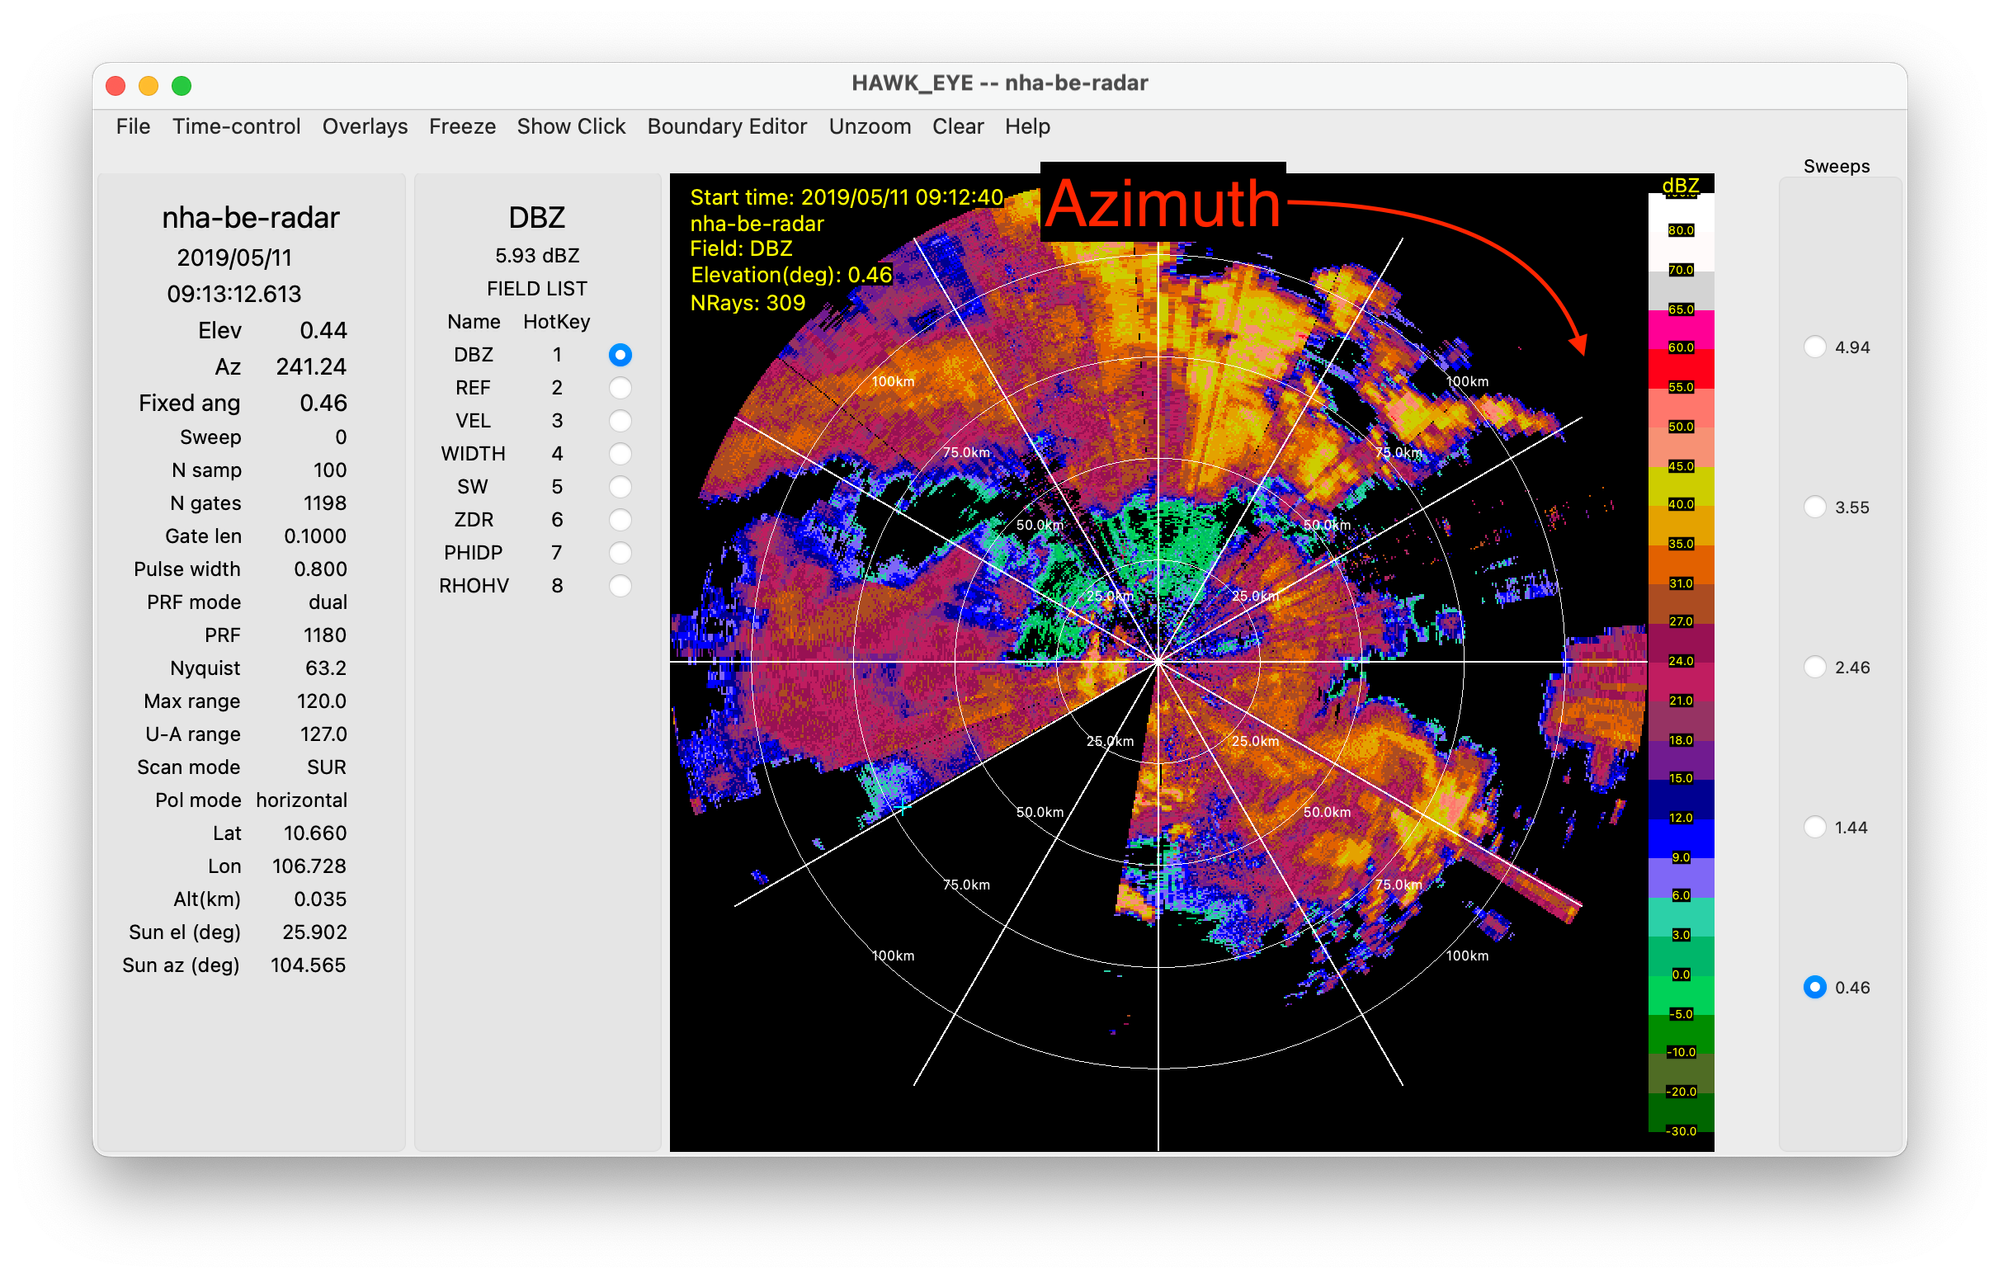
\includegraphics[width=0.8\textwidth]{Images/3.5-hawk-eye.png}
    \caption{HawkEye visualization tool}
    \label{fig:hawkeye}
\end{figure}

During our investigation, we also encountered a different set of tools that can interact with the radar files, called PyART.
When compared with LROSE-core, our team found that PyART contains many more advantages.

First, PyART is a Python library.
This means that it is easier to install and use, especially for people who are already familiar with Python.
Moreover, by supporting Python, our team can incorporate it into many popular ETL tools that use Python.
Take Apache Airflow as an example, instead of having to write a custom operator to call LROSE-core from the terminal,
we can use a Task to perform the same action with PyART. Doing so would reduce much of the complexity of the workflow.

\subsection{Visualizing data using PyART}
When installed, PyART also downloads another Python tool named Cartopy \cite{Cartopy}. This library provides many useful features
for our understanding of the data, such as the ability to plot the data on a map, or to convert the coordinates from one system to another.

Using these libraries, we can visualize our data directly from a Jupyter Notebook, similar to any other Python data visualization task. Also, by zooming out from the map, we can see the whole area that the radar covers, which is the district of Nha Be.

\begin{figure}[H]
    \centering
    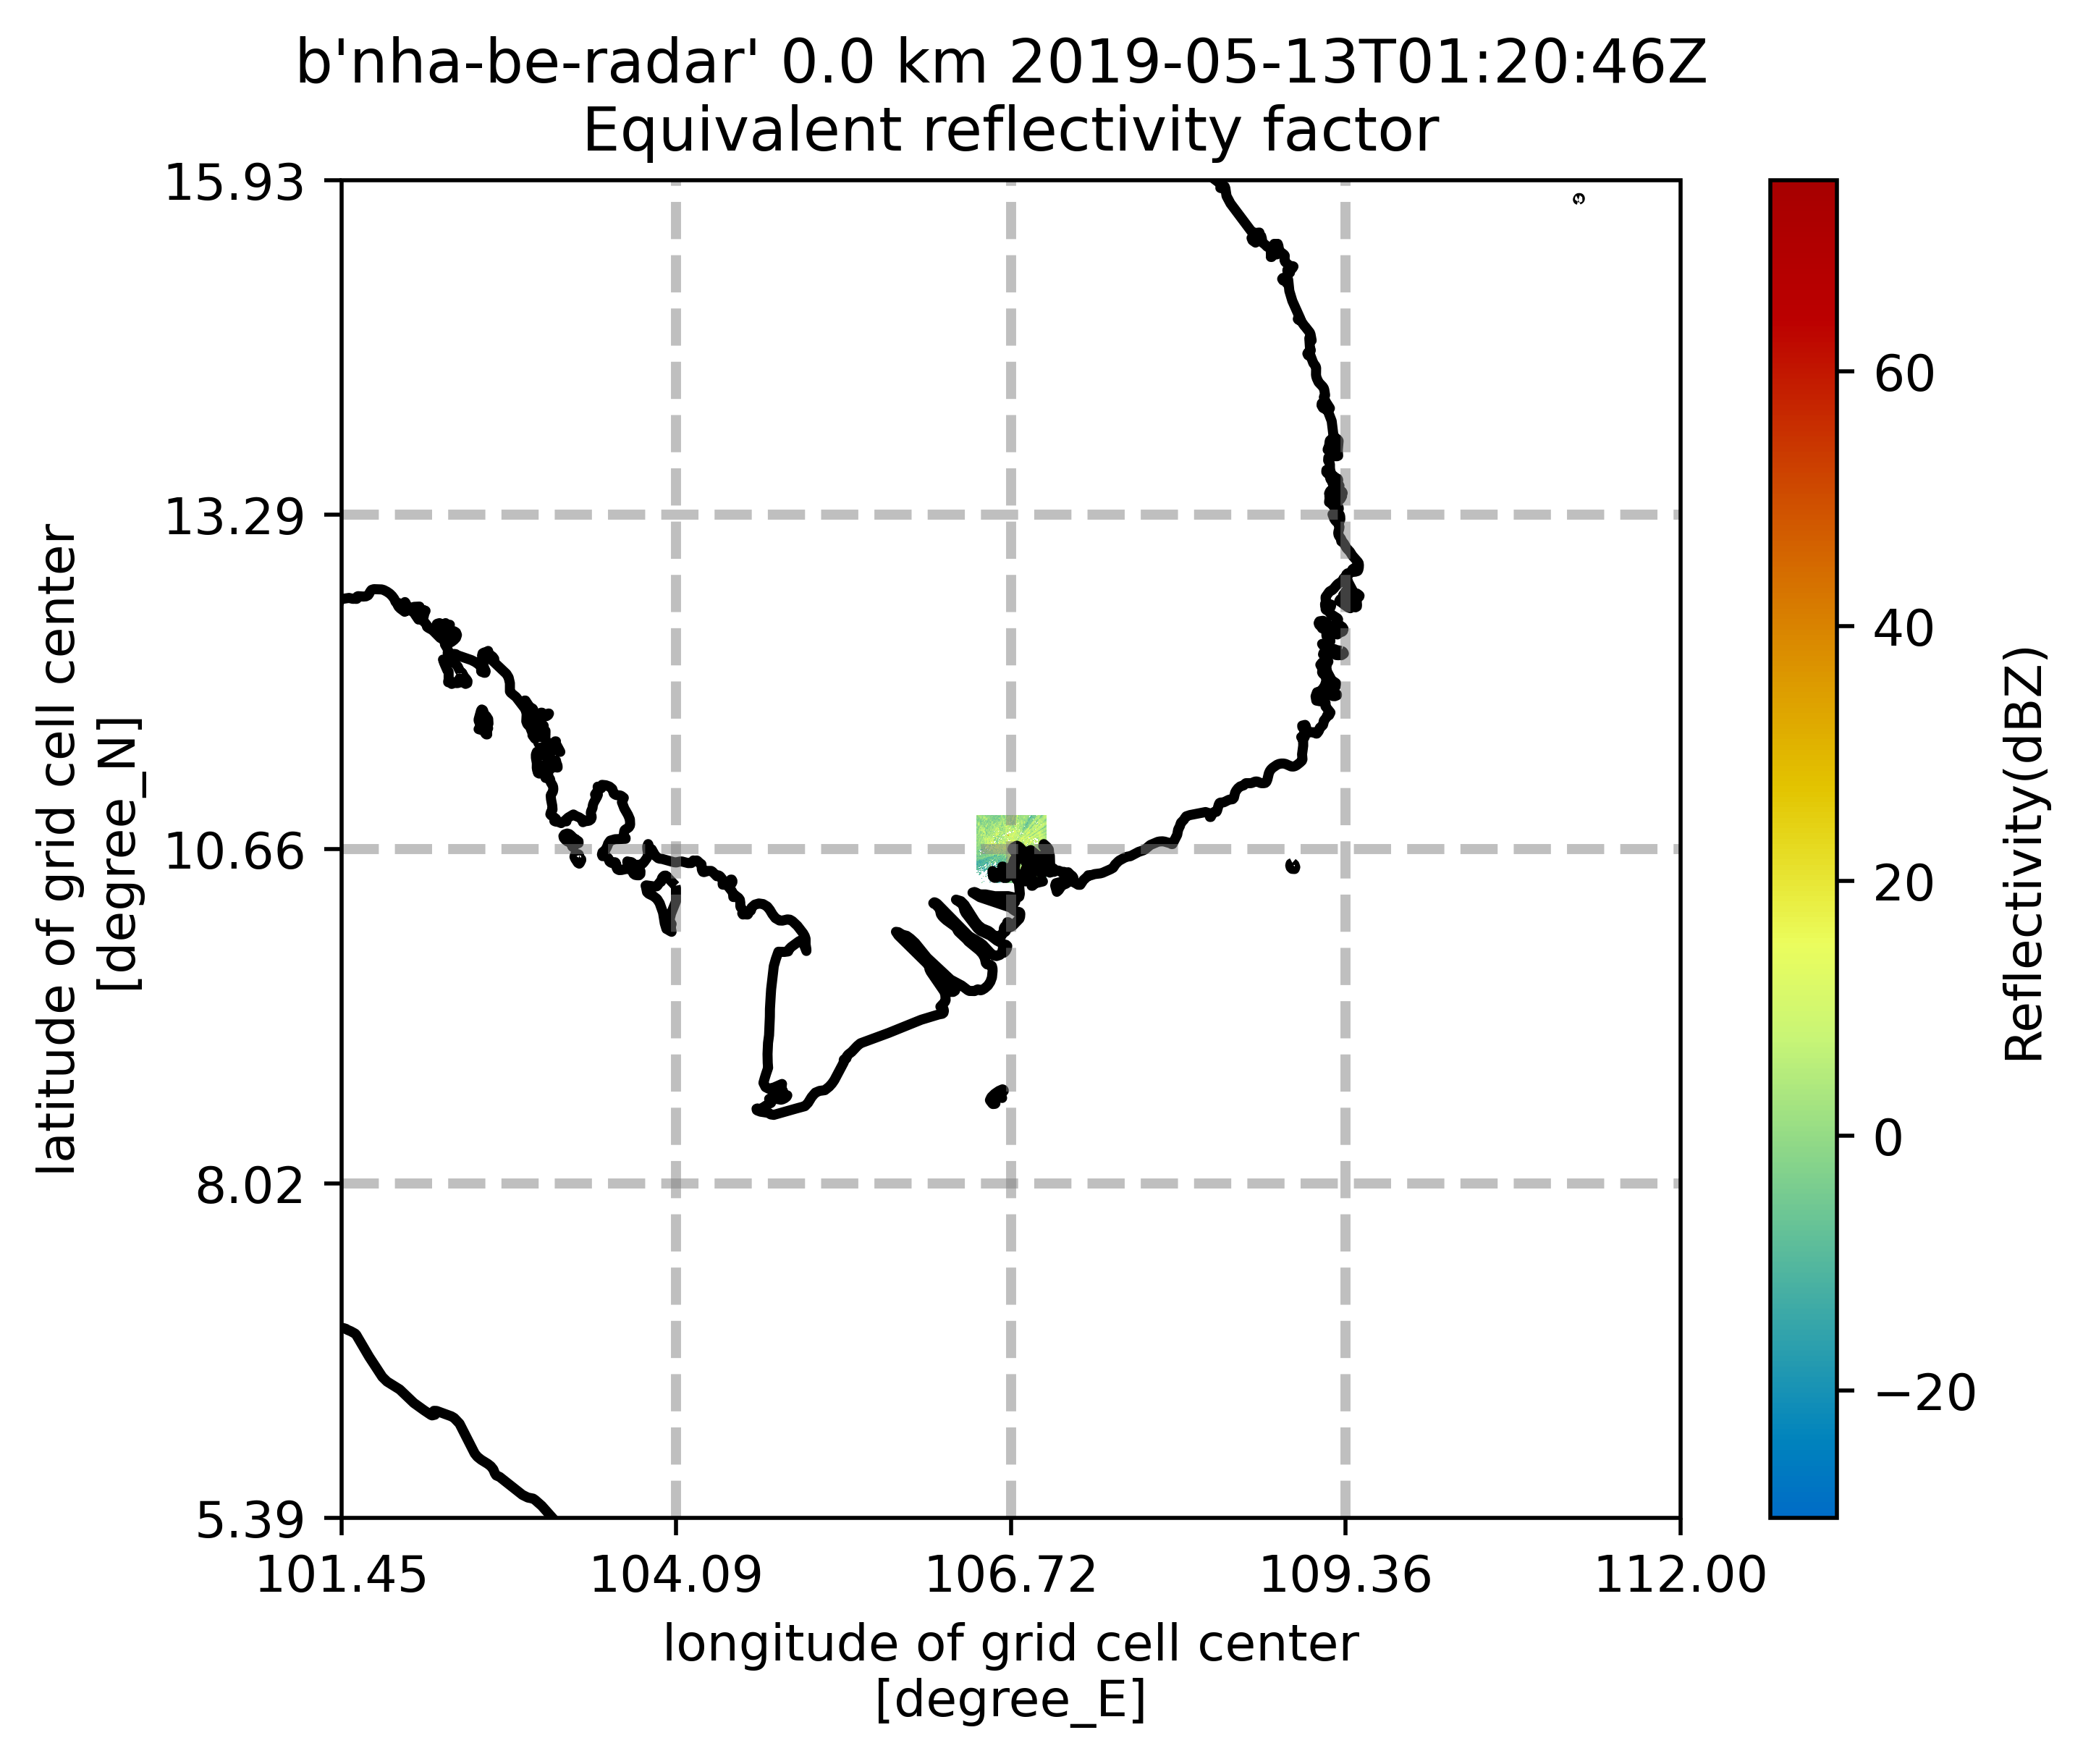
\includegraphics[width=0.8\textwidth]{Images/3.1-nha-be-radar-visualize-far.png}
    \caption{Data visualization of Nha Be radar - Map of Vietnam}
    \label{fig:nha-be-viz-far}
\end{figure}

